% Sección de resultados del proyecto final (modelo original BDL). Toda cifra sale de datos/ (generar.py).
\section{Resultados}\label{sec:resultados}

Esta sección compara el modelo original del proyecto, BDL (\emph{Boosting} con Desplazamiento Latente), con los modelos
del curso y con dos del estado del arte. Cada cifra sale de \texttt{generar.py}, que reproduce todas las tablas,
pruebas y figuras desde los resultados versionados del proyecto.

\subsection{Resumen del montaje experimental}\label{sec:res-montaje}

Los datos son los $48.723$ clientes sintéticos de COFINFAD \citep{munoz2025}, divididos al azar en
$38.978$ de entrenamiento y $9.745$ de prueba antes de mirar el objetivo; cuatro conjuntos públicos sirven de
contraste. La tarea principal es la regresión del puntaje continuo \cp; la métrica primaria es el RMSE y las
secundarias, MAE, MAPE y $R^2$. Todos los modelos usan el mismo preprocesamiento, las mismas particiones y $30$
evaluaciones de hiperparámetros en una validación anidada: tres repeticiones (semillas $42$, $43$ y $44$) de cinco
pliegues externos ($15$ particiones). El protocolo se registró en Git antes de los experimentos definitivos. Las referencias son $k$-NN, Ridge, Lasso, regresión bayesiana \citep{mackay1992}, árbol de decisión,
Random Forest, XGBoost \citep{chen2016xgboost}, SVR, EBM \citep{nori2019interpretml} y LightGBM \citep{ke2017}. La
regresión bayesiana se añadió después del protocolo, con los mismos pliegues; el SVR es lineal, porque el de kernel
RBF no escala a $38.978$ filas.

\subsection{Desempeño predictivo global}

Las Tablas~\ref{tab:desempeno} y~\ref{tab:prueba} resumen el desempeño en validación cruzada y en prueba. BDL obtiene
el mejor valor en todas las métricas de las dos: RMSE de $0{,}05887 \pm 0{,}00047$ en los pliegues, frente a
$0{,}05897 \pm 0{,}00047$ de XGBoost, el mejor benchmark, y $0{,}05912$ en prueba, frente a $0{,}05917$. Tiene menor
RMSE que cada una de las diez referencias en las $15$ particiones.

\begin{table}[tbp]
  \centering\scriptsize\setlength{\tabcolsep}{4pt}
  \caption{Desempeño en validación cruzada: media $\pm$ desviación en las 15 particiones externas (tres repeticiones de cinco pliegues), en orden de RMSE.}
  \label{tab:desempeno}
  \begin{tabular}{lcccc}
    \toprule
    Modelo & RMSE & MAE & $R^2$ & BDL gana en \\
    \midrule
    BDL (propuesto) & {\boldmath\textbf{$0{,}05887$ $\pm$ $0{,}00047$}} & {\boldmath\textbf{$0{,}04684$ $\pm$ $0{,}00034$}} & {\boldmath\textbf{$0{,}2303$ $\pm$ $0{,}0078$}} & -- \\
    XGBoost$^\dagger$ & \underline{$0{,}05897$ $\pm$ $0{,}00047$} & \underline{$0{,}04689$ $\pm$ $0{,}00032$} & \underline{$0{,}2277$ $\pm$ $0{,}0075$} & 15/15 \\
    LightGBM$^\dagger$ & $0{,}05899$ $\pm$ $0{,}00048$ & $0{,}04693$ $\pm$ $0{,}00034$ & $0{,}2271$ $\pm$ $0{,}0077$ & 15/15 \\
    EBM$^\dagger$ & $0{,}05903$ $\pm$ $0{,}00047$ & $0{,}04704$ $\pm$ $0{,}00033$ & $0{,}2262$ $\pm$ $0{,}0073$ & 15/15 \\
    Random Forest$^\dagger$ & $0{,}05913$ $\pm$ $0{,}00049$ & $0{,}04714$ $\pm$ $0{,}00035$ & $0{,}2234$ $\pm$ $0{,}0078$ & 15/15 \\
    Árbol de decisión$^\dagger$ & $0{,}05928$ $\pm$ $0{,}00048$ & $0{,}04741$ $\pm$ $0{,}00036$ & $0{,}2196$ $\pm$ $0{,}0081$ & 15/15 \\
    Lasso$^\dagger$ & $0{,}06181$ $\pm$ $0{,}00053$ & $0{,}05080$ $\pm$ $0{,}00035$ & $0{,}1515$ $\pm$ $0{,}0084$ & 15/15 \\
    Ridge$^\dagger$ & $0{,}06183$ $\pm$ $0{,}00053$ & $0{,}05076$ $\pm$ $0{,}00035$ & $0{,}1511$ $\pm$ $0{,}0085$ & 15/15 \\
    Regresión bayesiana$^\dagger$ & $0{,}06183$ $\pm$ $0{,}00053$ & $0{,}05075$ $\pm$ $0{,}00035$ & $0{,}1510$ $\pm$ $0{,}0086$ & 15/15 \\
    SVR lineal$^\dagger$ & $0{,}06185$ $\pm$ $0{,}00052$ & $0{,}05086$ $\pm$ $0{,}00033$ & $0{,}1505$ $\pm$ $0{,}0088$ & 15/15 \\
    k-NN$^\dagger$ & $0{,}06334$ $\pm$ $0{,}00052$ & $0{,}05129$ $\pm$ $0{,}00034$ & $0{,}1090$ $\pm$ $0{,}0044$ & 15/15 \\
    \bottomrule
  \end{tabular}
  \par\smallskip\begin{minipage}{0.97\linewidth}\scriptsize En negrita, el mejor de cada columna; subrayado, el segundo. $^\dagger$: la $t$ corregida de Nadeau-Bengio rechaza la igualdad con BDL ($p$ de Holm $<0{,}05$ sobre diez comparaciones). La última columna cuenta las particiones en que BDL tiene menor RMSE. La regresión bayesiana se añadió después del protocolo, con los mismos pliegues: Ridge, reajustado en ellos con sus hiperparámetros guardados, reproduce su RMSE de cada pliegue con una diferencia de $10^{-17}$; sus hiperparámetros se estiman por máxima evidencia.\end{minipage}
\end{table}


\begin{table}[tbp]
  \centering\scriptsize\setlength{\tabcolsep}{6pt}
  \caption{Desempeño en los 9.745 clientes de prueba, con el intervalo bootstrap BCa del 95~\% del RMSE (2000 réplicas).}
  \label{tab:prueba}
  \begin{tabular}{lccccc}
    \toprule
    Modelo & RMSE & IC 95~\% del RMSE & MAE & MAPE (\%) & $R^2$ \\
    \midrule
    BDL (propuesto) & {\boldmath\textbf{$0{,}05912$}} & [$0{,}05831$; $0{,}05992$] & {\boldmath\textbf{$0{,}04697$}} & {\boldmath\textbf{$15{,}96$}} & {\boldmath\textbf{$0{,}2197$}} \\
    XGBoost & \underline{$0{,}05917$} & [$0{,}05836$; $0{,}05996$] & \underline{$0{,}04706$} & \underline{$15{,}98$} & \underline{$0{,}2182$} \\
    LightGBM & $0{,}05918$ & [$0{,}05838$; $0{,}05997$] & $0{,}04707$ & \underline{$15{,}98$} & $0{,}2181$ \\
    EBM$^\ddagger$ & $0{,}05925$ & [$0{,}05845$; $0{,}06006$] & $0{,}04720$ & $16{,}03$ & $0{,}2161$ \\
    Random Forest$^\ddagger$ & $0{,}05931$ & [$0{,}05851$; $0{,}06011$] & $0{,}04728$ & $16{,}05$ & $0{,}2146$ \\
    Árbol de decisión$^\ddagger$ & $0{,}05944$ & [$0{,}05863$; $0{,}06025$] & $0{,}04750$ & $16{,}11$ & $0{,}2112$ \\
    Lasso$^\ddagger$ & $0{,}06166$ & [$0{,}06086$; $0{,}06251$] & $0{,}05072$ & $17{,}10$ & $0{,}1511$ \\
    Ridge$^\ddagger$ & $0{,}06167$ & [$0{,}06087$; $0{,}06253$] & $0{,}05069$ & $17{,}10$ & $0{,}1509$ \\
    Regresión bayesiana$^\ddagger$ & $0{,}06167$ & [$0{,}06088$; $0{,}06253$] & $0{,}05069$ & $17{,}10$ & $0{,}1508$ \\
    SVR lineal$^\ddagger$ & $0{,}06170$ & [$0{,}06091$; $0{,}06256$] & $0{,}05073$ & $17{,}10$ & $0{,}1499$ \\
    k-NN$^\ddagger$ & $0{,}06321$ & [$0{,}06234$; $0{,}06405$] & $0{,}05115$ & $17{,}28$ & $0{,}1080$ \\
    \bottomrule
  \end{tabular}
  \par\smallskip\begin{minipage}{0.97\linewidth}\scriptsize En negrita, el mejor de cada columna; subrayado, el segundo. $^\ddagger$: Diebold-Mariano-HLN sobre el error cuadrático de cada cliente rechaza la igualdad con BDL ($p$ de Holm $<0{,}05$). El MAPE solo se calcula en prueba, porque el protocolo no guardó los pronósticos de cada pliegue.\end{minipage}
\end{table}


La mejora absoluta sobre XGBoost es de $0{,}000099$ en los pliegues ($0{,}17$~\%) y de $0{,}000058$ en prueba
($0{,}10$~\%). Frente a los modelos lineales es de unos $0{,}0030$ ($4{,}8$~\%) y frente a $k$-NN, de $0{,}0045$
($7{,}1$~\%). La Figura~\ref{fig:folds} muestra dos grupos separados: los seis modelos de árboles, entre $0{,}0589$ y
$0{,}0593$, y los lineales y $k$-NN, por encima de $0{,}0618$. Dentro del primer grupo, las cajas se solapan casi por
completo y los intervalos BCa del RMSE en prueba \citep{efron1987} también.

\begin{figure}[tbp]
  \centering
  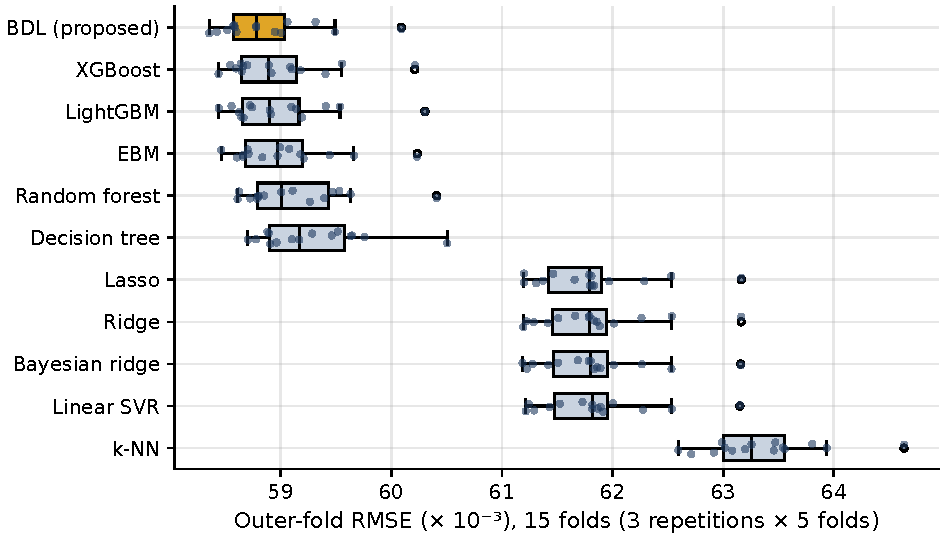
\includegraphics[width=\linewidth]{fig_folds}
  \caption{RMSE de cada modelo en las 15 particiones externas (tres repeticiones de cinco pliegues). Cada punto es una
  partición; BDL, en ámbar, tiene la mediana más baja. Los modelos de árboles forman un grupo y los lineales y $k$-NN,
  otro, unos $0{,}003$ más arriba.}
  \label{fig:folds}
\end{figure}

La ventaja no puede ser mucho mayor. El predictor óptimo, que conoce la fórmula del puntaje salvo la variable
excluida \ap, obtiene $0{,}05911$ en prueba y $0{,}05887$ en los pliegues: BDL queda a $0{,}00001$ en prueba y a
$0{,}000007$ en los pliegues de ese techo, y XGBoost, a $0{,}00007$ en prueba. El $R^2$ ronda $0{,}22$ porque la parte
del puntaje que depende de \ap{} no se puede predecir con los predictores disponibles.

La Figura~\ref{fig:regression} muestra esa estructura. El puntaje observado frente al pronosticado forma cinco bandas
paralelas, una por nivel de \ap. Los residuos de BDL se concentran en cinco picos estrechos separados por $0{,}05$:
el modelo separa casi por completo la señal observable del escalón latente. Los de XGBoost forman los mismos picos,
pero más anchos.

\begin{figure}[tbp]
  \centering
  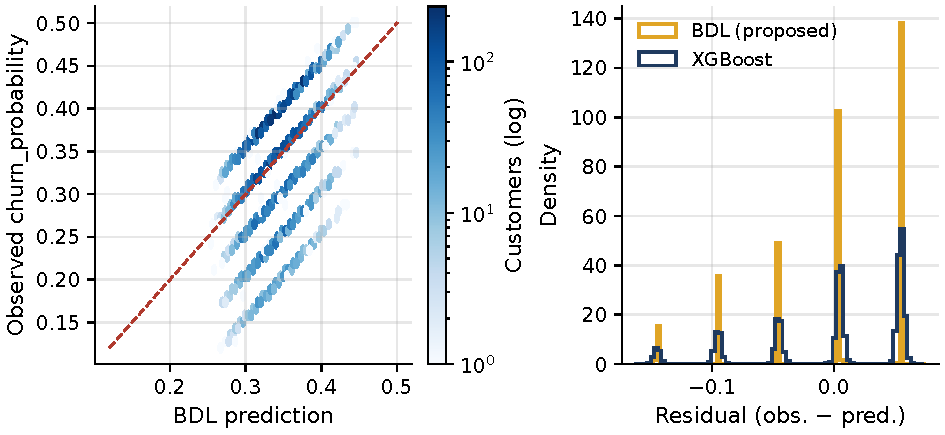
\includegraphics[width=\linewidth]{fig_regression}
  \caption{Izquierda: puntaje observado frente al pronóstico de BDL en los 9.745 clientes de prueba (escala logarítmica
  de conteos); la línea discontinua es la identidad. Las cinco bandas corresponden a los cinco niveles de la variable
  excluida \texttt{active\_products}. Derecha: densidad de los residuos de BDL y de XGBoost.}
  \label{fig:regression}
\end{figure}

\subsection{Resultados de las pruebas de significancia}

Se aplicó la combinación mínima que la guía exige para regresión tabular: la $t$ corregida de \citet{nadeau2003} sobre
las $15$ particiones, Diebold-Mariano \citep{diebold1995} con la corrección de \citet{harvey1997} sobre el error
cuadrático de cada cliente de prueba y la $t$ correlacionada bayesiana con región de equivalencia práctica (ROPE)
\citep{corani2015,benavoli2017}. Cada prueba se ajustó con Holm \citep{holm1979} sobre las diez referencias, con
$\alpha=0{,}05$. La ROPE es de $\pm0{,}0005$ en RMSE (cerca del $0{,}85$~\%), la misma de la versión anterior de esta
sección, fijada antes de calcular. Acompañan a cada $p$ la diferencia con su intervalo del $95$~\%, la $d$ de Cohen
\citep{cohen1988} y la $A_{12}$ de \citet{vargha2000}. La Tabla~\ref{tab:pruebas} y la Figura~\ref{fig:intervals}
reúnen los resultados.

\begin{table}[tbp]
  \centering\scriptsize\setlength{\tabcolsep}{1.8pt}
  \caption{Pruebas de significancia de BDL frente a cada referencia (combinación mínima de la guía para regresión tabular). $\Delta$: RMSE de la referencia menos RMSE de BDL, $\times 10^{3}$ (positivo: BDL se equivoca menos).}
  \label{tab:pruebas}
  \begin{tabular}{lcccccccc}
    \toprule
    Referencia & $\Delta$ pliegues [IC 95~\%] & $t$ corr. & $p_{\mathrm{Holm}}$ & DM-HLN & $p_{\mathrm{Holm}}$ & P(mejor / ROPE / peor) & $d$ & $A_{12}$ \\
    \midrule
    XGBoost & $+0{,}099$ [$0{,}053$; $0{,}144$] & $4{,}62$ & $0{,}001$ & $2{,}00$ & $0{,}092$ & $0{,}00$ / $1{,}00$ / $0{,}00$ & $0{,}21$ & $0{,}60$ \\
    LightGBM & $+0{,}119$ [$0{,}051$; $0{,}186$] & $3{,}77$ & $0{,}003$ & $1{,}92$ & $0{,}092$ & $0{,}00$ / $1{,}00$ / $0{,}00$ & $0{,}25$ & $0{,}60$ \\
    EBM & $+0{,}153$ [$0{,}068$; $0{,}239$] & $3{,}86$ & $0{,}003$ & $2{,}81$ & $0{,}015$ & $0{,}00$ / $1{,}00$ / $0{,}00$ & $0{,}33$ & $0{,}64$ \\
    Random Forest & $+0{,}260$ [$0{,}155$; $0{,}366$] & $5{,}30$ & $4{,}5 \times 10^{-4}$ & $3{,}51$ & $0{,}002$ & $0{,}00$ / $1{,}00$ / $0{,}00$ & $0{,}54$ & $0{,}72$ \\
    Árbol de decisión & $+0{,}407$ [$0{,}260$; $0{,}554$] & $5{,}93$ & $1{,}8 \times 10^{-4}$ & $4{,}78$ & $8{,}9 \times 10^{-6}$ & $0{,}10$ / $0{,}90$ / $0{,}00$ & $0{,}86$ & $0{,}76$ \\
    Lasso & $+2{,}939$ [$2{,}660$; $3{,}219$] & $22{,}55$ & $1{,}9 \times 10^{-11}$ & $13{,}70$ & $1{,}5 \times 10^{-41}$ & $1{,}00$ / $0{,}00$ / $0{,}00$ & $5{,}88$ & $1{,}00$ \\
    Ridge & $+2{,}954$ [$2{,}672$; $3{,}235$] & $22{,}50$ & $1{,}9 \times 10^{-11}$ & $13{,}75$ & $9{,}4 \times 10^{-42}$ & $1{,}00$ / $0{,}00$ / $0{,}00$ & $5{,}93$ & $1{,}00$ \\
    Regresión bayesiana & $+2{,}956$ [$2{,}672$; $3{,}240$] & $22{,}32$ & $1{,}9 \times 10^{-11}$ & $13{,}76$ & $9{,}1 \times 10^{-42}$ & $1{,}00$ / $0{,}00$ / $0{,}00$ & $5{,}94$ & $1{,}00$ \\
    SVR lineal & $+2{,}973$ [$2{,}682$; $3{,}265$] & $21{,}87$ & $1{,}9 \times 10^{-11}$ & $13{,}85$ & $3{,}0 \times 10^{-42}$ & $1{,}00$ / $0{,}00$ / $0{,}00$ & $6{,}03$ & $1{,}00$ \\
    k-NN & $+4{,}470$ [$4{,}174$; $4{,}767$] & $32{,}33$ & $1{,}5 \times 10^{-13}$ & $17{,}38$ & $1{,}2 \times 10^{-65}$ & $1{,}00$ / $0{,}00$ / $0{,}00$ & $9{,}02$ & $1{,}00$ \\
    \bottomrule
  \end{tabular}
  \par\smallskip\begin{minipage}{0.97\linewidth}\scriptsize $t$ corregida de Nadeau-Bengio sobre las 15 particiones (14 grados de libertad, intervalo con la misma varianza corregida); Diebold-Mariano con la corrección de Harvey-Leybourne-Newbold sobre el error cuadrático de los 9.745 clientes de prueba; $p$ ajustados con Holm sobre las diez referencias en cada prueba ($\alpha=0{,}05$). Prueba bayesiana: $t$ correlacionada con ROPE de $\pm0{,}0005$ en RMSE; probabilidades posteriores de que BDL sea mejor, equivalente o peor. $d$ de Cohen y $A_{12}$ de Vargha-Delaney entre los valores por pliegue (positivo y mayor que $0{,}5$ favorecen a BDL). BDL tiene menor RMSE que cada referencia en las 15 particiones.\end{minipage}
\end{table}


La $t$ corregida rechaza la igualdad frente a las diez referencias. Frente a XGBoost, la diferencia media es de
$0{,}099 \times 10^{-3}$, con intervalo $[0{,}053;\ 0{,}144] \times 10^{-3}$, $t=4{,}62$ y $p_{\mathrm{Holm}}=0{,}001$.
Diebold-Mariano rechaza frente a ocho: no lo hace frente a XGBoost ($p_{\mathrm{Holm}}=0{,}092$) ni frente a LightGBM
($0{,}092$). En prueba, la ventaja sobre XGBoost es de $0{,}058 \times 10^{-3}$ y su intervalo BCa,
$[0{,}005;\ 0{,}117] \times 10^{-3}$, apenas excluye el cero. En resumen, \textbf{BDL supera significativamente a ocho
de las diez referencias con las dos pruebas frecuentistas} ($p_{\mathrm{Holm}}<0{,}05$) y, frente a XGBoost y
LightGBM, solo con la $t$ corregida.

\begin{figure}[tbp]
  \centering
  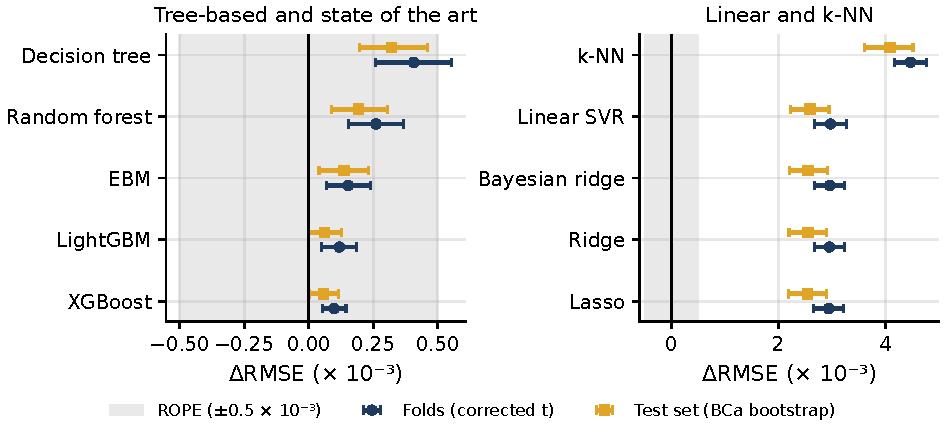
\includegraphics[width=\linewidth]{fig_intervals}
  \caption{Diferencia de RMSE de cada referencia menos BDL ($\times 10^{-3}$; positiva: BDL se equivoca menos), con
  su intervalo del 95~\%: en las 15 particiones (varianza corregida de Nadeau-Bengio, azul) y en los 9.745 clientes de
  prueba (bootstrap BCa, ámbar). La franja gris es la región de equivalencia práctica ($\pm 0{,}5 \times 10^{-3}$).
  A la izquierda, los modelos de árboles; a la derecha, los lineales y $k$-NN, en otra escala.}
  \label{fig:intervals}
\end{figure}

La prueba bayesiana distingue la significancia estadística de la relevancia práctica. BDL es mejor con probabilidad
posterior $1{,}000$ que los cuatro lineales y $k$-NN. Frente a XGBoost, LightGBM, EBM y Random Forest, la probabilidad
de que la diferencia caiga en la ROPE es de al menos $0{,}9999$: \textbf{BDL es prácticamente equivalente a esos
cuatro}. Frente al árbol, la posterior se reparte entre equivalencia ($0{,}903$) y superioridad ($0{,}097$). Las
diferencias frente a los modelos de árboles, de $0{,}10$ a $0{,}41 \times 10^{-3}$, equivalen a entre el $20$~\% y el
$81$~\% de la ROPE.

Los tamaños de efecto coinciden con esa lectura: $d=0{,}21$ y $A_{12}=0{,}60$ frente a XGBoost; $d=0{,}86$ y
$A_{12}=0{,}76$ frente al árbol; $d$ cercana a $6$ y $A_{12}=1$ frente a los lineales.

Las pruebas discrepan frente a XGBoost y LightGBM por la potencia, no por un error. La $t$ corregida usa $15$
métricas por pliegue y BDL gana en todas. Diebold-Mariano usa un solo conjunto de prueba, en el que la varianza del
error de cada cliente, dominada por el escalón latente, es enorme frente a una diferencia de RMSE de $0{,}000058$.
Wilcoxon de rangos con signo \citep{wilcoxon1945}, como verificación, rechaza frente a las diez
($p_{\mathrm{Holm}}=0{,}0006$), aunque comparte la dependencia entre pliegues. El \emph{Model Confidence Set}
\citep{hansen2011mcs} al $90$~\% sobre las pérdidas de prueba solo retiene a BDL; XGBoost y LightGBM salen con
$p=0{,}098$, justo en el borde.

El veredicto confirmatorio sigue siendo el del protocolo registrado, cuyas cuatro pruebas incluían dos en prueba:
frente a XGBoost rechazan Wilcoxon y la $t$ corregida, pero no la permutación pareada ($p_{\mathrm{Holm}}=0{,}092$) ni
el bootstrap BCa ($0{,}076$). Dos de cuatro no alcanzan las tres que exige la condición de superioridad, así que BDL
no se declara superior.

\begin{table}[tbp]
  \centering\scriptsize\setlength{\tabcolsep}{3pt}
  \caption{BDL en los cuatro conjuntos adicionales: RMSE medio en los cinco pliegues externos (semilla 42) del mejor benchmark de cada conjunto y de BDL, ventaja relativa (positiva si BDL es mejor), $p$ de la $t$ corregida y puesto entre los modelos.}
  \label{tab:conjuntos}
  \begin{tabular}{llccccc}
    \toprule
    Conjunto & Mejor benchmark & RMSE benchmark & RMSE BDL & Ventaja & $p$ ($t$ corr.) & Puesto \\
    \midrule
    Seguros médicos & EBM & $11.332$ & $11.435$ & $-0{,}90$~\% & $0{,}414$ & 8 de 11 \\
    Eficiencia energética & EBM & $2{,}2634$ & $2{,}3128$ & $-2{,}18$~\% & $0{,}474$ & 2 de 11 \\
    Abulón & Random Forest & $2{,}1293$ & $2{,}1683$ & $-1{,}83$~\% & $0{,}286$ & 5 de 11 \\
    Vivienda de California & LightGBM & $0{,}4426$ & $0{,}4645$ & $-4{,}95$~\% & $0{,}002$ & 3 de 11 \\
    \bottomrule
  \end{tabular}
  \par\smallskip\begin{minipage}{0.97\linewidth}\scriptsize Friedman con los 5 conjuntos como bloques y 11 modelos: $\chi^2=22{,}58$, $p=0{,}012$; Iman-Davenport $p=0{,}003$. Rango medio de BDL: $3{,}8$; diferencia crítica de Nemenyi: $6{,}75$ (Figura~\ref{fig:cd}).\end{minipage}
\end{table}


La Tabla~\ref{tab:conjuntos} y la Figura~\ref{fig:cd} amplían la comparación a cinco conjuntos. Friedman con la
corrección de Iman-Davenport \citep{demsar2006,iman1980} detecta diferencias entre los $11$ modelos ($\chi^2=22{,}58$,
$p=0{,}012$), pero la diferencia crítica de Nemenyi, $6{,}75$ rangos, no separa a ningún par de modelos. Los cinco
primeros son EBM ($2{,}8$), XGBoost ($3{,}4$), BDL ($3{,}8$), LightGBM ($4{,}0$) y Random Forest ($4{,}8$). BDL no es
mejor que el mejor benchmark en ninguno de los cuatro conjuntos adicionales, y es significativamente peor en Vivienda
de California ($-4{,}95$~\%, $p=0{,}002$). Con cinco conjuntos la potencia de Friedman es baja; la guía recomienda
diez o más.

\begin{figure}[tbp]
  \centering
  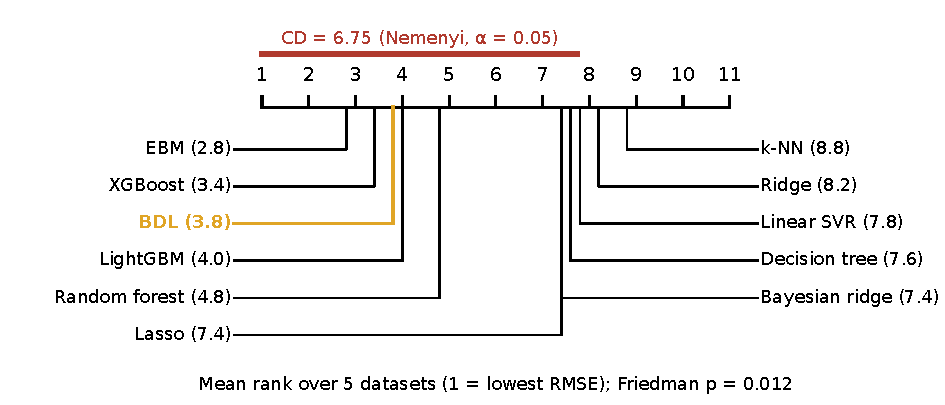
\includegraphics[width=\linewidth]{fig_cd}
  \caption{Diagrama de diferencia crítica con los cinco conjuntos de datos (COFINFAD y los cuatro adicionales) como
  bloques: rango medio de cada modelo por RMSE (1 = el mejor). Los modelos cuyos rangos difieren menos que la barra
  roja (Nemenyi, $\alpha=0{,}05$) no se distinguen; BDL, en ámbar, no se distingue de ninguno.}
  \label{fig:cd}
\end{figure}

\subsection{Resultados del estudio de ablación}

El componente propio de BDL es la mezcla latente de desplazamientos. La hipótesis registrada era que retirarla
($K=1$, un \emph{boosting} de mínimos cuadrados con los mismos árboles) aumenta el RMSE. La Tabla~\ref{tab:ablacion} y
la Figura~\ref{fig:ablation} aplican las mismas pruebas de la comparación principal.

\begin{table}[tbp]
  \centering\scriptsize\setlength{\tabcolsep}{1.8pt}
  \caption{Ablación de la mezcla latente en regresión: RMSE en los cinco pliegues externos de la semilla 42 y en prueba. Aporte: RMSE de la variante menos RMSE de BDL completo, $\times 10^{3}$ (positivo: la mezcla ayuda).}
  \label{tab:ablacion}
  \begin{tabular}{lccccccc}
    \toprule
    Variante & RMSE (pliegues) & Aporte [IC 95~\%] & $p$ ($t$ corr.) & P(ROPE) & RMSE prueba & Aporte prueba & $p$ (DM) \\
    \midrule
    BDL completo & $0{,}05887$ $\pm$ $0{,}00041$ & -- & -- & -- & $0{,}05912$ & -- & -- \\
    Sin mezcla ($K=1$) & $0{,}05898$ $\pm$ $0{,}00041$ & $+0{,}107$ [$0{,}008$; $0{,}205$] & $0{,}040$ & $0{,}9998$ & $0{,}05910$ & $-0{,}016$ & $0{,}623$ \\
    \midrule
    $K=1$ fijo & $0{,}05902$ $\pm$ $0{,}00040$ & $+0{,}142$ & -- & -- & -- & -- & -- \\
    $K=2$ fijo & $0{,}05897$ $\pm$ $0{,}00041$ & $+0{,}085$ & -- & -- & -- & -- & -- \\
    $K=3$ fijo & $0{,}05894$ $\pm$ $0{,}00039$ & $+0{,}053$ & -- & -- & -- & -- & -- \\
    $K=4$ fijo & $0{,}05889$ $\pm$ $0{,}00041$ & $+0{,}013$ & -- & -- & -- & -- & -- \\
    $K=5$ fijo & $0{,}05888$ $\pm$ $0{,}00041$ & $0{,}000$ & -- & -- & -- & -- & -- \\
    $K=6$ fijo & $0{,}05888$ $\pm$ $0{,}00041$ & $0{,}000$ & -- & -- & -- & -- & -- \\
    $K=8$ fijo & $0{,}05888$ $\pm$ $0{,}00041$ & $0{,}000$ & -- & -- & -- & -- & -- \\
    $K$ por BIC (final) & $0{,}05888$ $\pm$ $0{,}00041$ & -- & -- & -- & -- & -- & -- \\
    \bottomrule
  \end{tabular}
  \par\smallskip\begin{minipage}{0.97\linewidth}\scriptsize Las dos primeras filas son la ablación registrada, con las mismas pruebas de la comparación principal (hiperparámetros elegidos por la búsqueda en cada pliegue). Las demás vienen del análisis de sensibilidad: la configuración final con $K$ fijo o elegido por BIC, en los mismos pliegues y sin nueva búsqueda; son exploratorias y su aporte se mide frente a la última fila (positivo: la variante es peor).\end{minipage}
\end{table}


En los cinco pliegues de la semilla $42$, retirar la mezcla aumenta el RMSE en $0{,}107 \times 10^{-3}$, con
intervalo $[0{,}008;\ 0{,}205] \times 10^{-3}$, en los cinco pliegues y con $p=0{,}040$ en la $t$ corregida: la
hipótesis se confirma en validación cruzada. En prueba no se confirma: la variante sin mezcla queda
$0{,}016 \times 10^{-3}$ por delante ($p=0{,}62$ en Diebold-Mariano). La prueba bayesiana pone el aporte dentro de la
ROPE con probabilidad $0{,}9998$: con todos los datos, la mezcla mejora poco en la práctica.

Dos análisis exploratorios explican de dónde sale el aporte. Al fijar $K$, el RMSE baja con cada clase hasta cinco:
$+0{,}142$, $+0{,}085$, $+0{,}053$ y $+0{,}013 \times 10^{-3}$ para $K$ de $1$ a $4$, y $0$ desde $K=5$. El criterio
BIC elige $K=5$, el número real de niveles de \ap. Además, la ganancia de la mezcla crece cuando hay pocos datos:
$0{,}748 \times 10^{-3}$ ($1{,}3$~\%) con $3.118$ filas, $0{,}337$ con $7.796$, $0{,}187$ con $15.591$ y $0{,}142$
con $31.182$. Al restar del objetivo el escalón esperado, el \emph{boosting} aprende el índice con menos ruido, y eso
pesa más cuando hay pocas filas.

\begin{figure}[tbp]
  \centering
  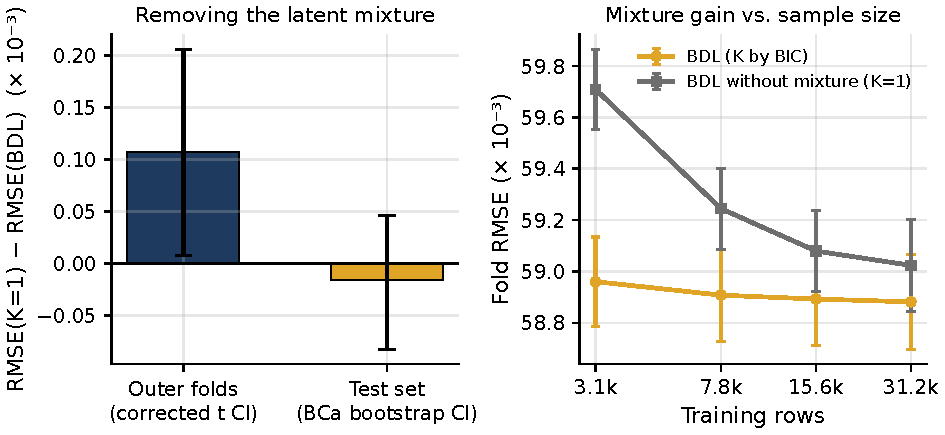
\includegraphics[width=\linewidth]{fig_ablation}
  \caption{Izquierda: aporte de la mezcla latente, RMSE sin mezcla ($K=1$) menos RMSE de BDL ($\times 10^{-3}$), con su
  intervalo del 95~\% en los cinco pliegues de la semilla 42 ($t$ corregida) y en prueba (bootstrap BCa). Derecha: RMSE
  por pliegue de BDL con y sin mezcla según el número de filas de entrenamiento (media $\pm$ error estándar en cinco
  pliegues).}
  \label{fig:ablation}
\end{figure}

\subsection{Sensibilidad y robustez}

La variación entre semillas es despreciable frente a las diferencias entre modelos (Tabla~\ref{tab:semillas}). Al
reajustar el modelo final con diez semillas, la desviación del RMSE en prueba es de $1{,}7 \times 10^{-6}$ en BDL,
frente a $5{,}0 \times 10^{-6}$ en XGBoost y $12{,}3 \times 10^{-6}$ en LightGBM. El orden de los modelos no depende de
la semilla.

\begin{table}[tbp]
  \centering\scriptsize\setlength{\tabcolsep}{3pt}
  \caption{Variación entre semillas del modelo final: RMSE en prueba al reajustar con diez semillas.}
  \label{tab:semillas}
  \begin{tabular}{lccc}
    \toprule
    Modelo & RMSE medio & Desviación ($\times 10^{-6}$) & Semillas \\
    \midrule
    BDL (propuesto) & $0{,}059116$ & $1{,}7$ & 10 \\
    XGBoost & $0{,}059171$ & $5{,}0$ & 10 \\
    LightGBM & $0{,}059183$ & $12{,}3$ & 10 \\
    EBM & $0{,}059259$ & $6{,}8$ & 10 \\
    Random Forest & $0{,}059306$ & $10{,}4$ & 10 \\
    \bottomrule
  \end{tabular}
\end{table}


La Figura~\ref{fig:sensitivity} resume las otras dos pruebas. A la derecha, al cambiar un hiperparámetro a la vez en
los mismos pliegues, $30$ de $34$ configuraciones quedan por delante de XGBoost con sus hiperparámetros finales
($0{,}05896$). Solo la tasa de aprendizaje de $0{,}05$ pierde más de una desviación entre pliegues ($0{,}05959$). A la
izquierda, la curva de aprendizaje: BDL con $3.118$ filas ($0{,}05896$) iguala a XGBoost con $31.182$.

Ante datos contaminados, BDL es el mejor de los tres \emph{boostings} en $8$ de $11$ escenarios. Pierde con ruido
gaussiano fuerte en el objetivo (desviación de $0{,}02$ o más) y con ruido fuerte en los predictores numéricos: la
mezcla supone escalones nítidos, y el ruido los desdibuja.

\begin{figure}[tbp]
  \centering
  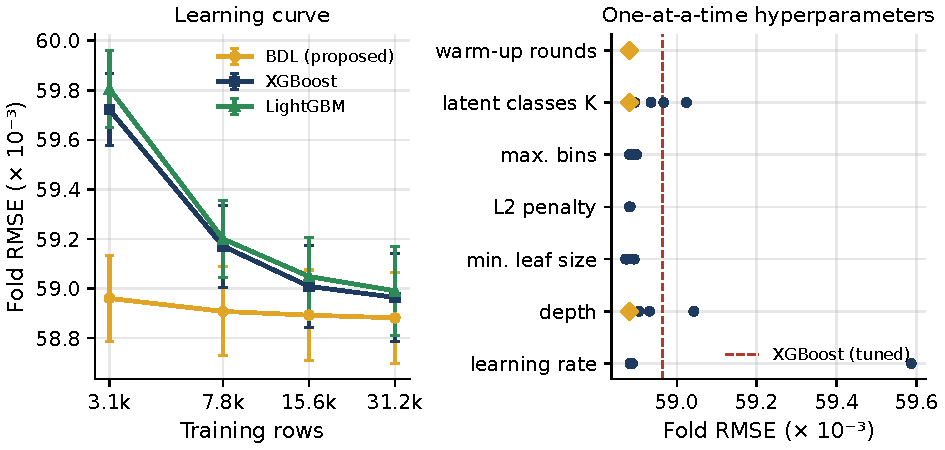
\includegraphics[width=\linewidth]{fig_sensitivity}
  \caption{Izquierda: curva de aprendizaje, RMSE por pliegue (media $\pm$ error estándar en cinco pliegues de la
  semilla 42) según las filas de entrenamiento, para BDL, XGBoost y LightGBM. Derecha: sensibilidad a cada
  hiperparámetro de BDL, cambiando uno a la vez respecto de la configuración final (rombo ámbar); la línea discontinua
  es XGBoost con sus hiperparámetros finales en los mismos pliegues.}
  \label{fig:sensitivity}
\end{figure}

\subsection{Costo computacional}

La Tabla~\ref{tab:costo} reúne el costo de cada modelo final. BDL tarda $5{,}8$~s en ajustarse con los $38.978$
clientes: $3{,}4$ veces lo de XGBoost ($1{,}7$~s), aunque menos que Random Forest ($11{,}2$~s) y la EBM ($25{,}5$~s).
Predice los $9.745$ clientes de prueba en $0{,}068$~s, unos $7$~$\mu$s por cliente, casi lo mismo que XGBoost. Su
memoria pico ($153$~MB) es la de XGBoost, y guarda $16.420$ parámetros en $149$~KB. En cuanto a si vale la pena: con todos los
datos, la ganancia de $0{,}17$~\% no justifica por sí sola triplicar el tiempo de ajuste. Sí lo justifica cuando los
datos son escasos (Figuras~\ref{fig:ablation} y~\ref{fig:sensitivity}) o cuando importa la estructura del error.

\begin{table}[tbp]
  \centering\scriptsize\setlength{\tabcolsep}{4pt}
  \caption{Costo computacional del modelo final de cada referencia: ajuste con todo el entrenamiento (38.978 clientes) e inferencia sobre los 9.745 de prueba (medias de diez semillas), memoria pico del ajuste, tamaño serializado y número de parámetros.}
  \label{tab:costo}
  \begin{tabular}{lccccc}
    \toprule
    Modelo & Ajuste (s) & Inferencia (s) & Memoria (MB) & Tamaño (KB) & Parámetros \\
    \midrule
    k-NN & $0{,}26$ & $4{,}889$ & $64$ & $6.295$ & 3.079.262 \\
    Regresión bayesiana & $0{,}35$ & $0{,}044$ & -- & $50$ & 79 \\
    Ridge & $0{,}41$ & $0{,}047$ & $67$ & $4$ & 79 \\
    Lasso & $0{,}42$ & $0{,}048$ & $65$ & $4$ & 79 \\
    LightGBM & $0{,}60$ & $0{,}062$ & $66$ & $46$ & 5.436 \\
    SVR lineal & $0{,}65$ & $0{,}048$ & $72$ & $4$ & 79 \\
    Árbol de decisión & $0{,}81$ & $0{,}047$ & $55$ & $6$ & 69 \\
    XGBoost & $1{,}69$ & $0{,}063$ & $154$ & $58$ & 3.899 \\
    BDL (propuesto) & $5{,}80$ & $0{,}068$ & $153$ & $149$ & 16.420 \\
    Random Forest & $11{,}25$ & $0{,}130$ & $66$ & $2.347$ & 86.158 \\
    EBM & $25{,}54$ & $0{,}055$ & $81$ & $1.032$ & 15.486 \\
    \bottomrule
  \end{tabular}
  \par\smallskip\begin{minipage}{0.97\linewidth}\scriptsize Equipo: AMD Ryzen 5 3500X (6 núcleos), 16 GB de RAM, Windows 11, sin GPU; Python 3.13.3. Parámetros: coeficientes en los modelos lineales; nodos en los árboles y conjuntos de árboles; celdas de las funciones de forma en la EBM; en BDL, las celdas de sus 78 funciones de forma (los 2.020 tocones se acumulan en ellas), los cortes y la mezcla; en k-NN, la matriz de entrenamiento que guarda. La memoria de la regresión bayesiana no se midió con el mismo procedimiento.\end{minipage}
\end{table}


\subsection{Interpretabilidad y análisis de errores}

La importancia por permutación en los clientes de prueba \citep{breiman2001} muestra que BDL y XGBoost usan las mismas
tres variables (Figura~\ref{fig:importance}). Barajar \texttt{age} aumenta el RMSE de BDL en $8{,}46 \times 10^{-3}$;
\texttt{app\_\allowbreak logins\_\allowbreak frequency}, en $5{,}56 \times 10^{-3}$, y
\texttt{satisfaction\_\allowbreak score}, en
$2{,}51 \times 10^{-3}$. Ninguna otra variable pasa de $0{,}04 \times 10^{-3}$. Es lo esperable en un conjunto
generado con reglas: el puntaje depende de esas tres variables y de \ap. BDL las aprovecha algo más que XGBoost
($7{,}95$, $5{,}30$ y $1{,}89 \times 10^{-3}$), porque aprende su índice sin el ruido del escalón.

\begin{figure}[tbp]
  \centering
  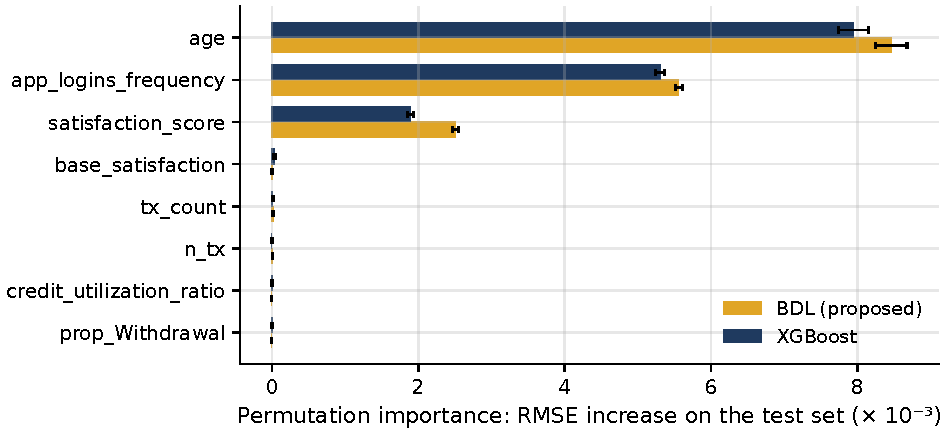
\includegraphics[width=\linewidth]{fig_importance}
  \caption{Importancia por permutación en los 9.745 clientes de prueba: aumento del RMSE al barajar cada variable
  original (media y desviación de cinco repeticiones), para BDL y XGBoost, con sus modelos finales de la semilla 43.
  Se muestran las ocho variables de mayor importancia.}
  \label{fig:importance}
\end{figure}

La mezcla de BDL es interpretable por sí misma. El modelo final tiene cinco clases con pesos $0{,}402$, $0{,}301$,
$0{,}149$, $0{,}098$ y $0{,}050$, separadas por $0{,}050$. Las proporciones reales de \ap{} en entrenamiento son
$0{,}402$, $0{,}301$, $0{,}149$, $0{,}099$ y $0{,}050$, con un escalón de $0{,}05$. \textbf{BDL recuperó la
distribución de la variable excluida sin verla.}

\begin{table}[tbp]
  \centering\scriptsize\setlength{\tabcolsep}{5pt}
  \caption{Error en prueba por subgrupo de clientes y por quintil del objetivo: BDL frente a XGBoost. Diferencia: RMSE de XGBoost menos RMSE de BDL, $\times 10^{3}$ (positiva: BDL se equivoca menos).}
  \label{tab:errores}
  \begin{tabular}{lcccc}
    \toprule
    Subgrupo & Clientes & RMSE BDL & RMSE XGBoost & Diferencia \\
    \midrule
    Todos & 9.745 & $0{,}05912$ & $0{,}05917$ & $+0{,}058$ \\
    \midrule
    Edad 29 & 1.643 & $0{,}05928$ & $0{,}05942$ & $+0{,}134$ \\
    Edad 30 & 1.581 & $0{,}06012$ & $0{,}06010$ & $-0{,}026$ \\
    Edad 44 & 1.598 & $0{,}05843$ & $0{,}05853$ & $+0{,}094$ \\
    Edad 45 & 1.576 & $0{,}05830$ & $0{,}05830$ & $-0{,}005$ \\
    Edad 59 & 1.631 & $0{,}05858$ & $0{,}05869$ & $+0{,}112$ \\
    Edad 60 & 1.716 & $0{,}05989$ & $0{,}05993$ & $+0{,}037$ \\
    \midrule
    \texttt{tx\_count} $>$ 500 (cola) & 134 & $0{,}06306$ & $0{,}06344$ & $+0{,}376$ \\
    \texttt{tx\_count} $\leq$ 500 & 9.611 & $0{,}05906$ & $0{,}05911$ & $+0{,}053$ \\
    \midrule
    Segmento inactive & 1.954 & $0{,}05874$ & $0{,}05875$ & $+0{,}016$ \\
    Segmento occasional & 3.852 & $0{,}05870$ & $0{,}05877$ & $+0{,}069$ \\
    Segmento power & 1.026 & $0{,}05885$ & $0{,}05894$ & $+0{,}085$ \\
    Segmento regular & 2.913 & $0{,}06000$ & $0{,}06006$ & $+0{,}063$ \\
    \midrule
    Quintil 1 del objetivo [$0{,}120$; $0{,}287$] & 1.954 & $0{,}09929$ & $0{,}09951$ & $+0{,}220$ \\
    Quintil 2 del objetivo [$0{,}287$; $0{,}337$] & 1.987 & $0{,}03802$ & $0{,}03722$ & $-0{,}791$ \\
    Quintil 3 del objetivo [$0{,}337$; $0{,}370$] & 1.910 & $0{,}03618$ & $0{,}03511$ & $-1{,}068$ \\
    Quintil 4 del objetivo [$0{,}370$; $0{,}400$] & 1.959 & $0{,}04607$ & $0{,}04567$ & $-0{,}399$ \\
    Quintil 5 del objetivo [$0{,}401$; $0{,}501$] & 1.935 & $0{,}05215$ & $0{,}05369$ & $+1{,}547$ \\
    \bottomrule
  \end{tabular}
\end{table}


El análisis de errores (Tabla~\ref{tab:errores}) señala dónde falla. Por subgrupo, BDL se equivoca menos que XGBoost
en $10$ de $12$, con la mayor ventaja en la cola de clientes con más de $500$ transacciones ($+0{,}376 \times 10^{-3}$).
Por quintil del objetivo, los dos modelos fallan más en los extremos: en el primero sobrestiman el puntaje en
$0{,}091$ y en el último lo subestiman en $0{,}050$. Es la regresión hacia la media que impone el escalón no
observable. BDL es mejor en los dos extremos ($+0{,}22$ y $+1{,}55 \times 10^{-3}$), justo en el de mayor riesgo, y
algo peor en los tres quintiles centrales (entre $-0{,}40$ y $-1{,}07 \times 10^{-3}$).

\subsection{Discusión, limitaciones y amenazas a la validez}

BDL funciona en COFINFAD porque el puntaje tiene la forma que el modelo supone: una función suave de tres variables
más un escalón aditivo que depende de una variable excluida. El \emph{boosting} aprende esa función sobre el objetivo
sin escalón, y por eso BDL queda a $0{,}00001$ del predictor óptimo en prueba. Es lo que se observa en los árboles con
efectos aleatorios \citep{hajjem2014,sigrist2022}: restar del objetivo un efecto de grupo antes de ajustar los árboles
los vuelve más eficientes; BDL lo hace sin observar el grupo. La ventaja es pequeña porque el techo está cerca: XGBoost
ya estaba a $0{,}00007$. En los conjuntos adicionales no hay un desplazamiento aditivo nítido (la búsqueda de
hiperparámetros eligió $K=1$ en los cuatro), y BDL se reduce a un \emph{boosting} programado desde cero, menos refinado
que XGBoost o LightGBM.

En clasificación, la tarea secundaria, BDL obtiene un AUC de $0{,}8313 \pm 0{,}0038$ en los pliegues (quinto de diez),
frente a $0{,}8333 \pm 0{,}0041$ de XGBoost, y ninguna prueba rechaza la igualdad. La superioridad no se cumple en
ninguna de las dos tareas.

Limitaciones. Los datos son sintéticos: las conclusiones no se trasladan a clientes reales. Cinco conjuntos
dan poca potencia a Friedman, y Diebold-Mariano descansa en un solo conjunto de prueba. La ROPE es una decisión del
equipo: con una más estrecha, la equivalencia práctica con los \emph{boostings} podría no sostenerse. La regresión
bayesiana, Diebold-Mariano y la prueba bayesiana se añadieron después del protocolo; son exploratorias y no cambian el
veredicto. Falta el SVR con kernel RBF. La auditoría no detectó fugas de
información.

La evidencia sugiere que BDL es el modelo más preciso en COFINFAD, con una ventaja estadísticamente detectable en
validación cruzada pero prácticamente equivalente a la de los mejores \emph{boostings}, y que esa ventaja no se
generaliza a otros conjuntos.
